% *********************************************************************
% © 2010–2021 Jeremy Sylvestre
%
% Permission is granted to copy, distribute and/or modify this document
% under the terms of the GNU Free Documentation License, Version 1.3 or
% any later version published by the Free Software Foundation; with no
% Invariant Sections, no Front-Cover Texts, and no Back-Cover Texts. A
% copy of the license is included in the appendix entitled “GNU Free
% Documentation License” that appears in the output document of this
% PreTeXt source code. All trademarks™ are the registered® marks of
% their respective owners.
%
% *********************************************************************

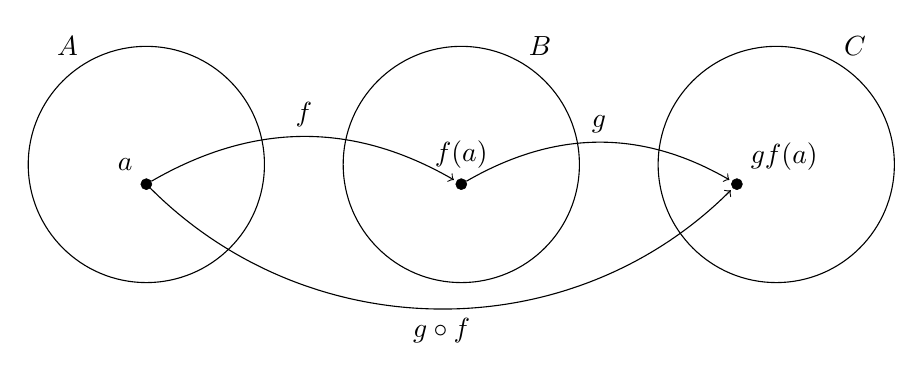
\begin{tikzpicture}[
	vertex/.style={ circle, draw, very thin, fill, inner sep=0pt, minimum size=4pt },
	vertexg/.style={ black!40!white, circle, draw, very thin, fill, inner sep=0pt, minimum size=4pt },
	vertexo/.style={ circle, draw, very thin, inner sep=0pt, minimum size=4pt }
]

\draw (6,0) circle (1.5cm);
\draw (2,0) circle (1.5cm);
\draw (-2,0) circle (1.5cm);
\node at (7,1.5) {$C$};
\node at (3,1.5) {$B$};
\node at (-3,1.5) {$A$};
\node at (-2,-0.25) (a) [vertex,label=above left:{$a$}] {};
\node at (2,-0.25) (b) [vertex,label=above:{$f(a)$}] {};
\node at (5.5,-0.25) (c) [vertex,label=above right:{$g\bbrac{f(a)}$}] {};
\draw[->,shorten >=1pt] (a) to [out=30,in=150] node[above] {$f$} (b);
\draw[->,shorten >=1pt] (b) to [out=30,in=150] node[above] {$g$} (c);
\draw[->,shorten >=1pt] (a) to [out=-45,in=-135] node[below] {$g \circ f$} (c);

\end{tikzpicture}
